\documentclass{article}
\usepackage{graphicx} % Required for inserting images
\usepackage[
    backend=biber,
    style=numeric,
]{biblatex}
\usepackage{url}

\addbibresource{bibfile.bib}

\title{HCS502: Assessment - AI/ML Project - 2310190}
\author{Thomas Morton}
\date{June 2025}

\begin{document}

\maketitle

\begin{abstract}
This study aims to explore and employ machine learning techniques in order to predict the cost of insurance premiums for an individual based on details about the driver as well as information about the vehicle. The research will also outline how each of these features affects the insurance premium for a driver. The data set being used has 1000 records containing the aforementioned data. This dataset will be used to train and analyse both simple and multivariate regression models, clustering algorithms and neural networks. Data preprocessing was carried out on the data, which consisted of normalisation in the form of scaling and anomaly identification.

\end{abstract}

\newpage

\section{Introduction}
Car insurance and its workings are a mystery to many. It traditionally relies on analysis and experts in the domain of car insurance to make assumption and asses the risk of certain drivers and vehicles and set a driver's insurance premium based on this knowledge and experience. In the modern world, with comparison sites and insurers in the 100's or even 1000's, artificial intelligence (AI), along with machine learning (ML), probably already run the business side of most insurers on the market. Although it may seem unfair to let these algorithms control the prices, they use data-driven methods which is trained on raw facts from the world of motoring. This technology offers an automated solution, saving the companies a lot of money in training individual staff members on the risk factors to look out for in a person. 

This project investigates how effective a simple regression algorithm, using one factor, or a multivariate algorithm, using multiple factors, can be used to predict car insurance premiums based on the information provided. Linear regression is known for its interpretability and efficiency in a computational sense\cite{scikit_LR}, which allows for easy identification of trends and displaying the correlation between key factors. In applying these models to a structured dataset, this study aims to explore how effectively insurance premiums can be predicted, which will allow the assessment of the model accuracy and evaluate how this can also present the risk of over-fitting to the data.

Understanding the relationship between these factors is imperative to the research into the workings of insurance company pricing structures. This research seeks to provide more transparent pricing and show the factors that have the biggest impact on an insurance policy.

\newpage
\section{Dataset and Pre-processing}

\begin{figure}[h]
\centering
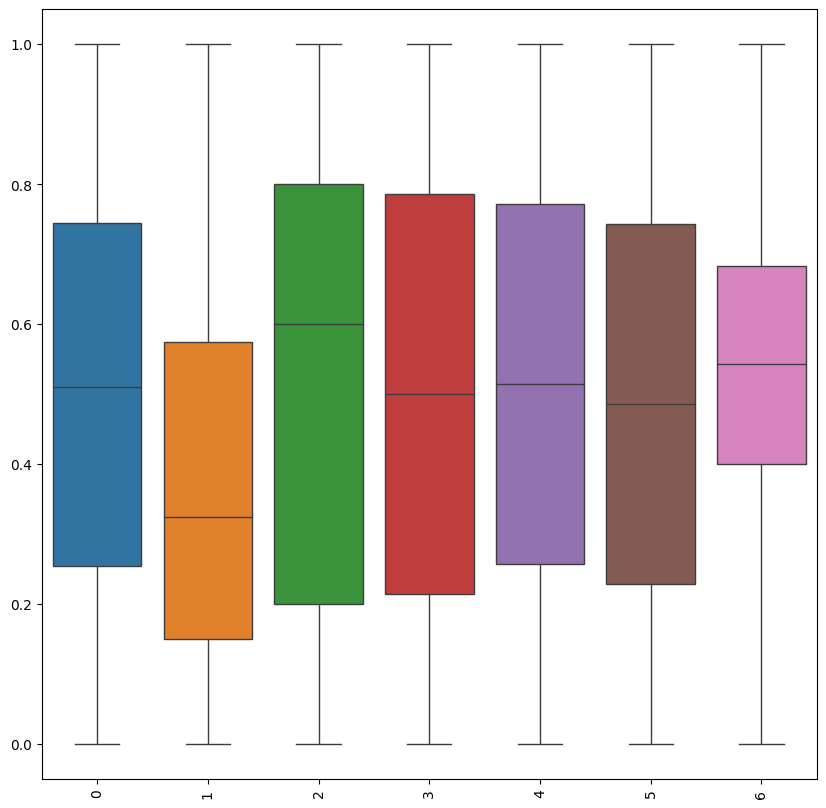
\includegraphics[width=0.8\textwidth]{boxplot.png}
\caption{Boxplot of Normalised Variables}\label{fig:boxplot}
\end{figure}

The dataset was sources from Kaggle.com and provides an array of information including the details about a driver, their vehicle and the insurance premium they were quoted because of this\cite{Sriram_2025}. The dataset consists of 1000 rows of data containing numerical features along with the insurance price. Thee features include; Driver Age, Driver Experience, Previous Accidents, Annual Mileage (KM), Car Manufacturing Year, Car Age and finally, the target variable, Insurance Premium in US dollars.  

To ensure the data was of a high enough quality, there was some initial exploratory analysis that took place in the form of normalisation, box plots and statistical summary. The initial check was to make sure where were no null values in the data, of which there are none as shown below in the output of an `isnull().sum()' check. SKlearn's standard scaler \cite{scikit_scaler} was used to normalise the data for the boxplots which makes it a lot easier to plot and pick out any outliers, of which there are none in this instance. Due to the nature of our data, all of the variables are integers or floats, this was confirmed by using 'df.dtypes' against the imported dataframe.

\begin{verbatim}
Driver Age                   0
Driver Experience            0
Previous Accidents           0
Annual Mileage (x1000 km)    0
Car Manufacturing Year       0
Car Age                      0
Insurance Premium ($)        0
dtype: int64
\end{verbatim}





\newpage
\section{Exploratory Data Analysis (EDA)}

\begin{figure}[h]
\centering
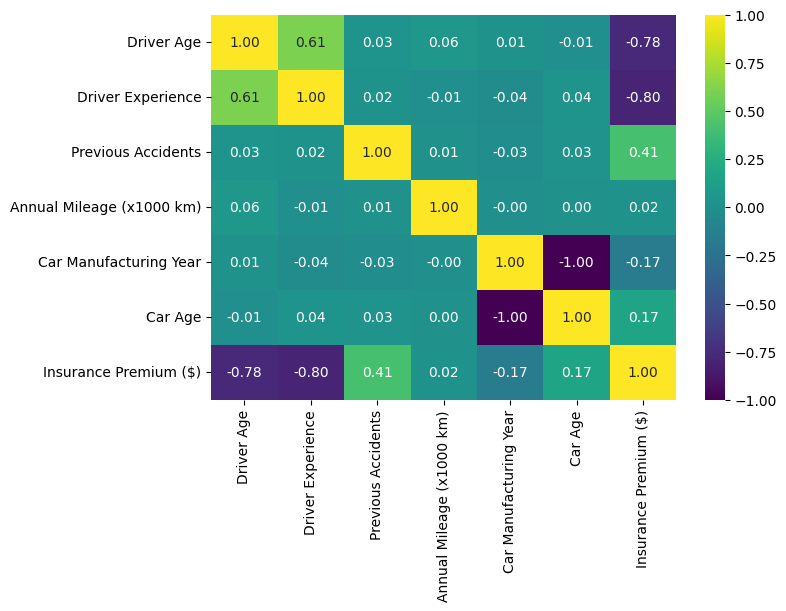
\includegraphics[width=0.8\textwidth]{heatmap.png}
\caption{Correlation Heatmap of All Features}\label{fig:heatmap}
\end{figure}

Using seaborn makes it simple to view a heatmap of the correlation between all of the variables. This is shown in figure \ref{fig:heatmap} comparing the relationip of any of the features against any other feature. In this heatmap it points out the strong negative correlations between 'Driver Age' and 'Driver Experience', these show a negative corealtion of -0.78 and -0.80 respectively. This suggests that older and more expericenced drivers are considered safer drivers which in turn allows them to have a lower insurance premium. This alligns with general risk assesment principles that expericenced drivers tend to be safer and older drivers often more sensible on the road. 

As expected, previous accidents seems to have a fairly strong positive correlation against insurance premiums. This implies that the more accidents that a driver has, the more at risk they are on the road. This again aligns with general risk assessment principles that drivers that have accidents more often, are more likely to have another accident in future. Other features in our dataset showed weaker and more negligable correlations, meaning that the correlation is not as strong and these have less of an effect on the price of car insurance. It would be interesting to see if other factors were added to this dataset, how much effect they would have. Such as engine size (cc), engine power (bhp), driveterrain layout (AWD, FWD, RWD), however those are not available for this dataset.

\newpage
\section{Modelling and Evaluation}

Choosing a model to use for the application requires some testing of various models and evaluating the results. Some obvious choices are simple linear regression and multivariate regression. K-nearest neighbor regression is also useful for seperating data into different groups, however for predicting a continuous value such as insurance premiums, linear regression is the more appropirate. Dispite this, this section will cover all aforementioned to ensure no opportunities for appropirate models are missed.

\subsection{Simple Linear Regression}
Linear regression models aim to establish a linear relationship between input features $x_i$ and the continuous target variable $y$ (insurance premium), typically expressed as:

$$
\hat{y} = \beta_0 + \sum_{i=1}^p \beta_i x_i
$$

where $\beta_0$ is the intercept and $\beta_i$ are the coefficients learned from data\cite{hastie_09_elements-of.statistical-learning}.



\begin{figure}[h]
\centering
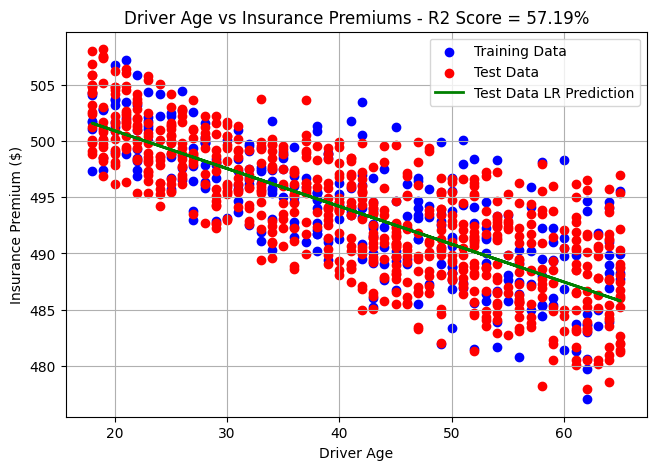
\includegraphics[width=0.8\textwidth]{age_insurance_LR.png}
\caption{Regression Line: Driver Age vs Insurance Premium}\label{fig:regression_age}
\end{figure}
In the above figure \ref{fig:regression_age}, the relationship between driver age and insurance premium is shown. Although the data is not perfectly linear, it does show a trend that as the driver age increases, the insurance premium decreases.This aligns with the negative correlation seen in the heatmap. The R2 score for this model was 57.19\% which indicates that 57\% of of the price variance in insurance premiums can be explained by the age of the driver. This is a fairly low score for a linear regressions model, however this is to be expected as it is commonly known that there are many factors that can affect the price of car insurance premiums.
\subsection{Multivariate Regression}
\begin{figure}[h]
\centering
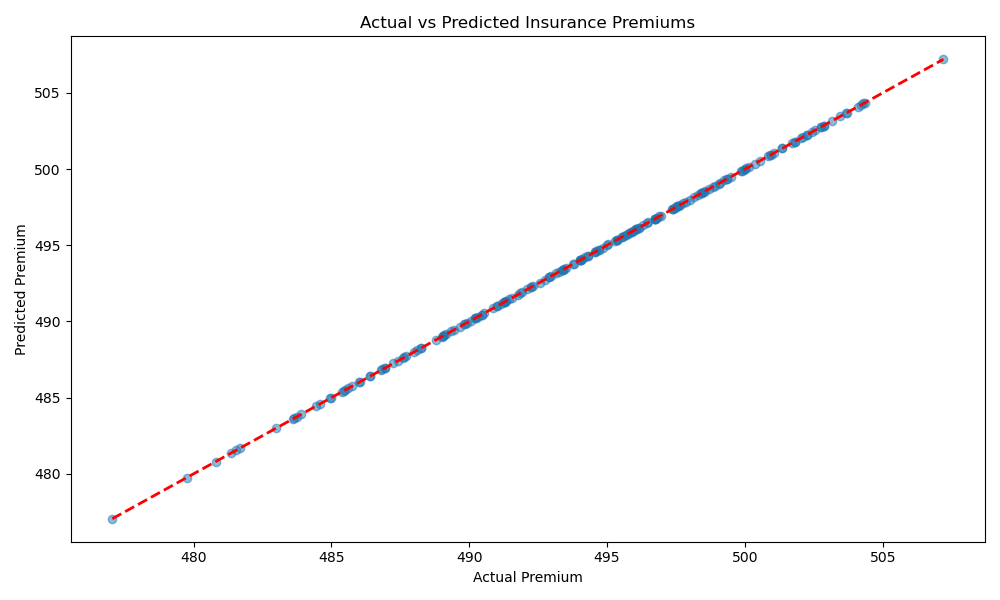
\includegraphics[width=0.8\textwidth]{actual_vs_predicted.png}
\caption{Actual vs Predicted Premiums (Multivariate Model)}\label{fig:multivariate_regression}
\end{figure}

Multivariate regression is just like the simple linear regression, however, it uses multiple features to predict the target variable. In this model, it was trained on all of the features in the dataset, minus 'Vehicle Manufacturing Year' as this was not required due to the fact that 'Vehicle Age' in years was already included. The X values used included: 'Driver Age', 'Driver Experience', 'Previous Accidents', 'Annual Mileage (x1000 km)', and 'Car Age'. The model was once again trained using the \texttt{scikit-learn} model\cite{scikit_LR}. In the above figure \ref{fig:multivariate_regression}, the actual insurance prices are plotted against the predicted insurance prices. The model unusually predicts the prices perfectly, with an R squared score of 1.0, meaning that the model was 100\% correct in all of it's predictions. This indicated that the dataset being used may have been artificially generated using a similar model, or that the dataset is just too small to be able to generalise. Either way, the perfect score of this model makes it an obvious choice for the model to use for the application.

\newpage

\subsection{K-Nearest Neighbors Regression}

\begin{figure}[h]
\centering
\includegraphics[width=0.8\textwidth]{knn_regression.png}
\caption{K-Nearest Neighbors Regression Results}\label{fig:knn_regression}
\end{figure}

K-Nearest neighbors (KNN) is a model that predicts the target variable based on the average of it's "Nearest Neighbors", hence the name. This model is useful for clustering data into groups, however it is not as useful for predicting a continuous value such as insurance premiums. However, it is still worth testing to see how it may perform against the other models. The model show in figure \ref{fig:knn_regression} shows that the model has a Mean Squared Error (MSE) of 1.35, which is a fairly low score in terms of MSE. This, along with the R squared score of 0.96 does still indicate that the model is fairly accurate, however it is not as accurate as the perfect multivariate regression model.

\subsection{Model Comparison}

\begin{itemize}
\item Simple linear regression provides interpretability for individual feature but lower accuracy.
\item Multivariate regression achieves very high performance on synthetic data but raises questions about generalisability if presented with another less synthetic dataset.
\item K-Nearest Neighbors regression offers a balance between interpretability and accuracy, however it may struggle with larger datasets and continuous target variables.
\end{itemize}

\newpage
\section{Software Environment \& Application}

\begin{figure}[h]
\centering
    \begin{minipage}{0.45\textwidth}
        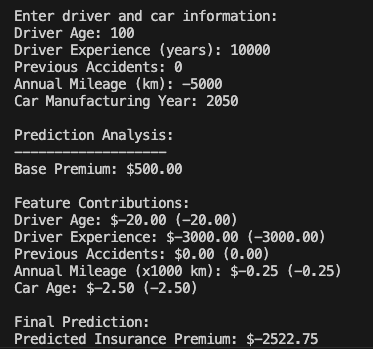
\includegraphics[width=0.8\textwidth]{negative_price.png}
        \caption{Negative Annual Mileage Effect on Insurance Premium}\label{fig:negative_mileage}
    \end{minipage}
    \hfill
    \begin{minipage}{0.45\textwidth}
        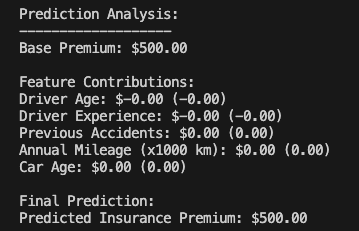
\includegraphics[width=0.8\textwidth]{base_price.png}
        \caption{Base Price of Insurance Premium}\label{fig:base_price}
    \end{minipage}
\end{figure}

The machine learning pipeline was implemented in Python 3.13.2 and Anaconda using very common python libraries including \texttt{pandas} for data manipulation in the way of creating dataframes and analysing the data, \texttt{scikit-learn} for modeling the data, and \texttt{matplotlib} and \texttt{seaborn} for visualizations such as graphs and charts.

The application created is an insurance price predictor that allows a user to input their details and retrieve a predicted insurance premium based on the data provided which matches the features in the dataset. Once the user has entered their details into the application, it will use the multivariate regression model that was chosen previously, to predict the insurance prices. The application will then produce a result that displays the predicted premium, but also the factors that were used to produce this result. I will display how much each facture contributed to the final price by using the coefficients from the multivariate regression model. 

The application also uses the y-intercept of the model to provide a base price of the insurance premiums of \$500. This seems to be common practice in the insurance industry to have a base price for insurance premiums. This base price was testing by entering all user details as 0 (setting car year to 2025) and the model returned a price of \$500. As a result of this, validation checks were implemented to ensure that the user does not enter any values that would not make sense in the context of purchasing insurance. For example, a driver cannot be younger that 17 years old, and the experience cannot be more than the driver age minus 17, this is because it was based on the minimum driving age in the UK, which is 17 years old. The application also checks that the annual mileage and the car age is not negative, otherwise this has a drastic effect on the insurance premiums, which can be see on the figures \ref{fig:negative_mileage} \ref{fig:base_price}.


\newpage
\section{Results Analysis}

\newpage
\section{Ethical Considerations}

The use of machine learning for predicting car insurance premiums introduces several ethical concerns:

\textbf{Fairness and Bias:} 

\textbf{Data Privacy:} 

\textbf{Transparency:} 

\textbf{Accountability:} 

\newpage
\section{Conclusion}

\newpage

\printbibliography

\end{document}